
La aplicación solicitada era la siguiente: \textit {“Pedir el precio de un producto y el monto que ha dado un cliente, posteriormente calcular el número mínimo de monedas a dar en el vuelto si se tienen las monedas de la siguiente denominación: 2.00, 1.00, 0.50, 0.25, 0.10.”}

Con esto en mente y siguiendo con el patrón MVC y la metodología de diseño de Atomic Design, se tiene la siguiente estructura dentro de la carpeta “coins”:

\begin{figure}[H]
    \centering
    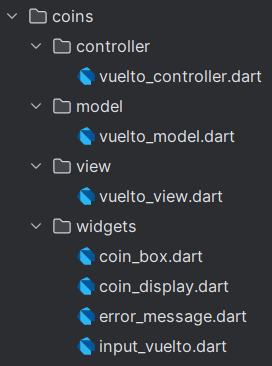
\includegraphics[width=0.6 \textwidth, height=8cm, keepaspectratio]{ej12/cap1.png}
    \caption{Estructura de archivos en proyecto coins}
    \label{fig:ej12il1}
\end{figure}

A continuación se mostrarán cada uno de los archivos y su respectiva funcionalidad.

\textbf{vuelto model}

Esta clase define dos variables: “precio” y “monto”. Dichas variables se utilizarán para realizar el cálculo del vuelto. Para ello también se cuenta con una variable constante, que no es más que un array de 5 elementos con las denominaciones en centavos de las monedas de cambio. Esto es así para evitar tener problemas de operaciones de punto flotante.

\begin{center}
\begin{lstlisting}
const MONEDAS = [200,100,50,25,10];

class VueltoModel {

  final double precio;
  final double monto;

  VueltoModel(this.precio, this.monto);

  (List<int>, double) obtenerMonedas() {
    int cambio = ((monto - precio) * 100).round();

    var monedasVuelto = [0,0,0,0,0];
    int resto = cambio;

    int i = 0;
    while(i<5) {
      if(resto == 0){
        break;
      }

      if((resto - MONEDAS[i]) < 0) {
        i++;
        continue;
      }

      resto -= MONEDAS[i];
      monedasVuelto[i]++;
    }

    return (monedasVuelto, resto/100);
  }
}
\end{lstlisting}
\end{center}

Se tiene la función “obtenerMonedas()” que regresa dos valores, una lista con las monedas de cambio y un valor restante, porque puede haber casos donde no se alcance a dar todo el vuelo en su totalidad.

Dicha función para calcular el vuelto, primero obtiene el cambio (en centavos) que se tiene que dar. Luego se itera sobre cada denominación de moneda de mayor a menor y se le resta del monto total que se tiene que devolver con cada iteración así hasta cubrir todo el array (las 5 denominaciones). Finalmente se devuelve el array actualziado con las monedas de cambio y el valor del resto, que se lo divide para 100.

\textbf{vuelto controller}

Esta clase hace uso del “modelo” anterior. Consta de un único método “calcularCambio()” el cual recibe 2 argumentos de tipo String, que corresponden al precio y el monto que provienen de los campos de texto de la interfaz. Este método regresa dos valores, una lista con las monedas de cambio y un mensaje de error, para que pueda ser mostrado en pantalla.

\begin{center}
\begin{lstlisting}
class VueltoController{
  (List<int>, String) calcularCambio(String precioProd, String montoUsr) {...}
}
\end{lstlisting}
\end{center}

A coninuación, se realizan varias verificaciones de casos donde existan errores en la entrada de datos. Si llega a ocurrir, se devuelve una lista con ceros y el respectivo mensaje de error.

\begin{center}
\begin{lstlisting}
    // verificar que los campos estén llenados
    if(precioProd.isEmpty || montoUsr.isEmpty) {
      return (List.filled(5, 0), "Llene todos los campos para continuar");
    }

    final precio = double.tryParse(precioProd);
    final monto = double.tryParse(montoUsr);

    // verificar que sean valores double
    if(precio == null || monto == null) {
      return (List.filled(5, 0), "Ingrese un valor numérico");
    }

    // verificar que no hayan valores negativos
    if(monto < 0 || precio < 0) {
      return (List.filled(5, 0), "¡No pueden haber valores negativos!");
    }

    // verificar que el monto sea mayor que el precio
    if(monto < precio) {
      return(List.filled(5, 0), "¡El monto ingresado es menor al precio del producto!");
    }
\end{lstlisting}
\end{center}

Una vez verificados los errores de ingreso de datos, se procede a utilizar el VueltoModel para ejecutar el algoritmo para calcular el cambio en monedas llamando a su método “obtenerMonedas()”.

\begin{center}
\begin{lstlisting}
    // si no hay errores en el ingreso a datos calular el vuelto con el Model
    final vuelto = VueltoModel(precio, monto);
    final (monedas, resto) = vuelto.obtenerMonedas();
\end{lstlisting}
\end{center}

Se hace una comprobación final, puesto que dadas las denominaciones de monedas, puede haber casos donde no se pueda cubrir todo el cambio. Por ello se comprueba si hay resto, de ser el caso se devuelve la cantidad de monedas correspondiente junto con un mensaje con la cantidad de falta dar.

\begin{center}
\begin{lstlisting}
    // caso especial, si no se pudo dar todo el vuelto
    if(resto != 0) {
      return (monedas,"Faltan por dar \$${resto}" );
    }

    // si se pudo dar todo el vuelto, regresar sin mensaje de error
    return (monedas, "");
\end{lstlisting}
\end{center}

Si no hay ningún problema se regresa la cantidad de monedas con un mensaje de error en blanco.

\textbf{widgets}

\begin{itemize}
    \item \textbf{input vuelto}
\end{itemize}

Este widget es muy sencillo. Consta de un controlador (el que maneja el texto que ingresa al Input) y de un texto que se muestra como retroalimentación (label). 

Luego en términos de personalización se ajusta el widget TextField para que solo tome valores numéricos, que muestre un borde sutil y el texto de retroalimentación.

\begin{center}
\begin{lstlisting}
class InputVuelto extends StatelessWidget {
  final TextEditingController ctrl;
  final String label;

  InputVuelto({
    super.key,
    required this.ctrl,
    required this.label
  });

  @override
  Widget build(BuildContext context) {
    return TextField(
      controller: ctrl,
      keyboardType: TextInputType.number,
      decoration: InputDecoration(
        labelText: label,
        border: OutlineInputBorder(),
      ),
    );
  }
}
\end{lstlisting}
\end{center}

\begin{itemize}
    \item \textbf{coin display}
\end{itemize}

Este widget muestra un contenedor con forma circular con el valor de la denominación de la moneda y al lado muestra la cantidad respectivamente. Por tal motivo tiene dos atributos “coinValue” y “value”.

\begin{center}
\begin{lstlisting}
class CoinDisplay extends StatelessWidget {
  final String coinValue;
  final int value;

  CoinDisplay({
    super.key,
    required this.coinValue,
    required this.value
  });
\end{lstlisting}
\end{center}

Puesto que los elementos se ubican de forma horizontal, se utiliza un widget Row en primer lugar. Luego como primer elemento se tiene a un “Container” al cual se le da forma de círculo con la propiedad “shape: BoxShape.circle” y adentro del mismo muestra un texto correspondiente al valor de la denominación de la moneda.

\begin{center}
\begin{lstlisting}
  @override
  Widget build(BuildContext context) {
    return Row(
      mainAxisSize: MainAxisSize.min,
      children: [
        // Contenedor en forma de círculo
        Container(
          width: 80,
          height: 80,
          decoration: BoxDecoration(
            shape: BoxShape.circle,
            color: Colors.white,
            border: Border.all(
              color: Colors.black,
              width: 3,
            ),
          ),
          child: Center(
            child: Text(
              coinValue,
              style: TextStyle(
                fontWeight: FontWeight.bold,
                fontSize: 16,
                color: Colors.black,
              ),
              textAlign: TextAlign.center,
            ),
          ),
        ),
\end{lstlisting}
\end{center}

Luego se tiene un pequeño espaciado horizontal con \lstinline{SizedBox(width: 16),}. Finalmente se muestra un texto plano que corresponde a la cantidad que se tiene que dar de esa moneda.

\begin{center}
\begin{lstlisting}
Text(
    "$value",
    style: TextStyle(
      fontSize: 24,
      fontWeight: FontWeight.w500,
      color: value !=0 ? Colors.amber[800] : Colors.black,
    ),
),
\end{lstlisting}
\end{center}

\begin{itemize}
    \item \textbf{coin box}
\end{itemize}

Este widget utiliza el “CoinDisplay” anterior para mostrar las diferentes monedas en pantalla. Para ello se tiene un array del monto de cada moneda, el cual es pasado en su constructor.

\begin{center}
\begin{lstlisting}
import 'coin_display.dart';

class CoinBox extends StatelessWidget {
  final List<int> monedas_vuelto;

  const CoinBox({super.key, required this.monedas_vuelto});
\end{lstlisting}
\end{center}

La distribución de los elementos es de la siguiente manera. Un pequeño título al inicio, seguido de 4 widgets de CoinDisplay en una cuadrícula 4x4 y un CoinDisplay centrado en la parte del último. Por tal motivo al construir el widget, se utiliza “Column” al inicio para generar la disposición de los elementos de forma vertical.

\begin{center}
\begin{lstlisting}
  @override
  Widget build(BuildContext context) {
    return Column(
      children: [
        Center(
          child: Text(
            "Cantidad de monedas a dar",
            style: TextStyle(fontSize: 20, fontWeight: FontWeight.bold),
          ),
        ),
\end{lstlisting}
\end{center}

Para ubicar los CoinDisplay de forma contigua en horizontal, se utiliza el widget “Row”, al cual se le pasan dos widgets de CoinDisplay, cada uno se lo inicializa con el nombre de la denominación de la moneda y su valor correspondiente de cambio dado por el atributo “monedas\_vuelto” declarado al inicio.

\begin{center}
\begin{lstlisting}
SizedBox(height: 24,),

    Row(
      mainAxisAlignment: MainAxisAlignment.spaceEvenly,
      children: [
        CoinDisplay(coinValue: "\$2.00", value: monedas_vuelto[0]),
        CoinDisplay(coinValue: "\$1.00", value: monedas_vuelto[1]),
      ],
    ),

    SizedBox(height: 24,),

    Row(
      mainAxisAlignment: MainAxisAlignment.spaceEvenly,
      children: [
        CoinDisplay(coinValue: "\$0.50", value: monedas_vuelto[2]),
        CoinDisplay(coinValue: "\$0.25", value: monedas_vuelto[3]),
      ],
    ),

    SizedBox(height: 24,),

    Center(
      child: CoinDisplay(coinValue: "\$0.10", value: monedas_vuelto[4]),
    ),
\end{lstlisting}
\end{center}


\begin{itemize}
    \item \textbf{error message}
\end{itemize}

Este widget muestra un mensaje de error en pantalla cuando se necesario. Por tal motivo puede ocupar espacio en pantalla o no. Para ello primero se necesita que se le pase un texto a mostrar, el cual puede llegar a ser nulo.

\begin{center}
\begin{lstlisting}
class ErrorMessage extends StatelessWidget {
  final String? errorText;

  const ErrorMessage({
    super.key,
    this.errorText,
  });
\end{lstlisting}
\end{center}

En primera instancia, al construir el widget, se verifica si el texto suministrado es nulo o simplemente se encuentra vacío. De ser el caso, se regresa un \lstinline{SizedBox.shrink()}, para que no ocupe espacio en la pantalla.

\begin{center}
\begin{lstlisting}
  @override
  Widget build(BuildContext context) {
    if (errorText == null || errorText!.isEmpty) {
      return const SizedBox.shrink();
    }
\end{lstlisting}
\end{center}

Si hay un texto que mostrar se arma el widget como tal. Para ello, se parte desde un “Padding” que contiene un “Container” que será el que tendrá el mensaje de error y tendrá un color rojo característico, junto con bordes redondeados.

\begin{center}
\begin{lstlisting}
return Padding(
  padding: const EdgeInsets.all(16),
  child: Container(
    decoration: BoxDecoration(
      color: Color.fromRGBO(255, 0, 0, 0.1),
      borderRadius: BorderRadius.circular(12),
      border: Border.all(
        color: Color.fromRGBO(255, 0, 0, 0.1),
        width: 1.5,
      ),
    ),
\end{lstlisting}
\end{center}

El Container, tendrá un widget Padding que a su vez tendrá un widget “Expanded”. Este último es importante porque se ajustará según el espacio lo requiera. Esto porque el Expanded tendrá un widget “Text” con el mensaje de error y como este puede ser muy largo, el tamaño del contenedor se tiene que ajustar. 

\begin{center}
\begin{lstlisting}
child: Padding(
  padding: const EdgeInsets.all(16),
  child: Row(
    children: [
      Expanded(
        child: Text(
          errorText!,
          style: const TextStyle(
            color: Colors.red,
            fontSize: 18,
            fontWeight: FontWeight.w500,
          ),
          textAlign: TextAlign.start,
        ),
      ),
    ],
  ),
),
\end{lstlisting}
\end{center}

Dicho texto se encuentra estilizado, siendo de color rojo y orientado de tal manera para que pueda ser visualizado correctamente.

\textbf{vuelto view}

Esta es la vista principal en la que el usuario interactuará.Puesto que su contenido se actualiza dinámicamente, se lo define como un “StatefulWidget”, por lo que se especifica una clase para manejar su estado.

\begin{center}
\begin{lstlisting}
class VueltoPage extends StatefulWidget {
  @override
  State<VueltoPage> createState() => _VueltoPageState();
}
\end{lstlisting}
\end{center}

Dicha clase define varias variables:
\begin{itemize}
    \item Los controladores para los Inputs de precio y conto.
    
    \item El controlador del vuelto para llamar al algoritmo y manejar errores.
    
    \item Las monedas de vuelto y el mensaje de error que se mostrarán en pantalla.
\end{itemize}

\begin{center}
\begin{lstlisting}
class _VueltoPageState extends State<VueltoPage> {
  // declarar controladores
  final precioCtrl = TextEditingController();
  final montoCtrl = TextEditingController();
  final vueltoCtrl = VueltoController();

  // declarar variables
  var monedas_vuelto = [0,0,0,0,0];
  String msgError = "";
\end{lstlisting}
\end{center}

Luego se tiene un método privado “\_calcularVuelto()” que se encargará de actualizar el estado del widget; es decir, actualizará sus las variables respecto al monto de monedas y al mensaje de error.

\begin{center}
\begin{lstlisting}
void _calcularVuelto() {
    // Obtener valores usando el controllador
    final (monVuel, err) = vueltoCtrl.calcularCambio(precioCtrl.text, montoCtrl.text);

    // actualizar el estado según los valores
    setState(() {
      monedas_vuelto = monVuel;
      msgError = err;
    });
}
\end{lstlisting}
\end{center}

Luego se define el diseño a presentar, por lo que se utiliza un “Scaffold” para definir la estructura principal de una “AppBar”.

\begin{center}
\begin{lstlisting}
@override
Widget build(BuildContext context) {
  return Scaffold(
    appBar: AppBar(
      title: Text("Vuelto Mínimo"),
      backgroundColor: Colors.blue[900],
      foregroundColor: Colors.white,
      centerTitle: true,
    ),
\end{lstlisting}
\end{center}

Finalmente se hace uso de los widgets definidos anteriormente para generar la pantalla principal dentro del \lstinline{body} del Scaffold.

\begin{center}
\begin{lstlisting}
child:  Column(
  crossAxisAlignment: CrossAxisAlignment.stretch,
  children: [
    Text(
      "Ingrese el precio del producto y el monto a pagar",
      style: TextStyle(fontSize: 16, fontWeight: FontWeight.bold),
    ),
    SizedBox(height: 12,),
    InputVuelto(ctrl: precioCtrl, label: "precio (2 decimales)"),
    SizedBox(height: 12,),
    InputVuelto(ctrl: montoCtrl, label: "monto (2 decimales)"),
    SizedBox(height: 12,),
    ElevatedButton(
        onPressed: _calcularVuelto,
        child: Text("Calcular")
    ),
    ErrorMessage(errorText: msgError),
    SizedBox(height: 18,),
    CoinBox(monedas_vuelto: monedas_vuelto),
  ],
),
\end{lstlisting}
\end{center}